\chapter{機構の実装}
\label{chp:first}

\section{マテリアルの検討}
\label{sec:paragraph}
今回開発する3DプリンターはFDM方式の改良である.FDM方式では,常温で固体の物質を加熱し柔らかくしてから押し出している.
水のプリントの場合は液体を押し出し,押し出し後に冷却して固体にする.
プラスチックと比べ液体の場合,押し出されるときのマテリアルの粘度が印刷精度や印刷時間に違いをもたらしているのではと考える.

今回開発した氷をマテリアルとした3Dプリンターの材料として水に砂糖を混ぜて粘度を上げたものを用意した.
砂糖はどこでも手に入りかつ安価で扱いも簡単であるため,今回の実験に採用した,
水と砂糖の割合は 1:3 のものを用意した.水との粘度の比較を図4.1に示す.

\begin{figure}[H]
  \centering
  \includegraphics[width=15truecm]{./fig/sugar.jpg}
  \caption{砂糖を添加した割合ごとの水}
% \url{http://www.this.is.sample.url/} % Web上のデータの場合、参照先URLを明記
  \label{fig:stage}
\end{figure}


\section{予備実験}
\label{sec:paragraph}

水に砂糖を加え粘度を上げた液体で造形を行う方式の実証を行った.

初めに,3D プリンターとして自動化させる前に,水の粘度が造形物の造形速度,造形精度,オーバーハングの造形に影響を与えるのか調査を行った. 
造形の仕組みは図4.2のようになっている.実験の装置は, 保温のため一番下に発泡スチロールの容器を用意した.
その上に-196 度の液体窒素を十分に注ぎ,さらにその上からアルミトレーを沈める.
それにより,アルミトレーも液体窒素に近い温度まで冷やされ,そこに注射器を使い水あめと水の中間の粘度の水をたらすことで,冷やされた水が氷に変わる.
冷やされた氷の温度は 0 度よりも低く,その上に水をたらすことで氷が積層される. 

\begin{figure}[H]
  \centering
  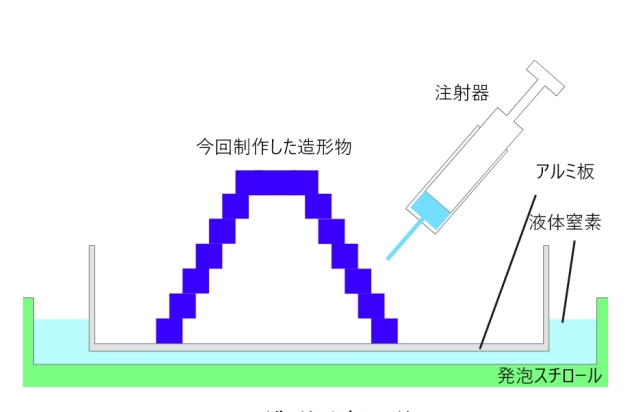
\includegraphics[width=10truecm]{./fig/yobi2.jpg}
  \caption{設計図と造形した形}
% \url{http://www.this.is.sample.url/} % Web上のデータの場合、参照先URLを明記
  \label{fig:yobitamesi}
\end{figure}

\begin{figure}[H]
  \centering
  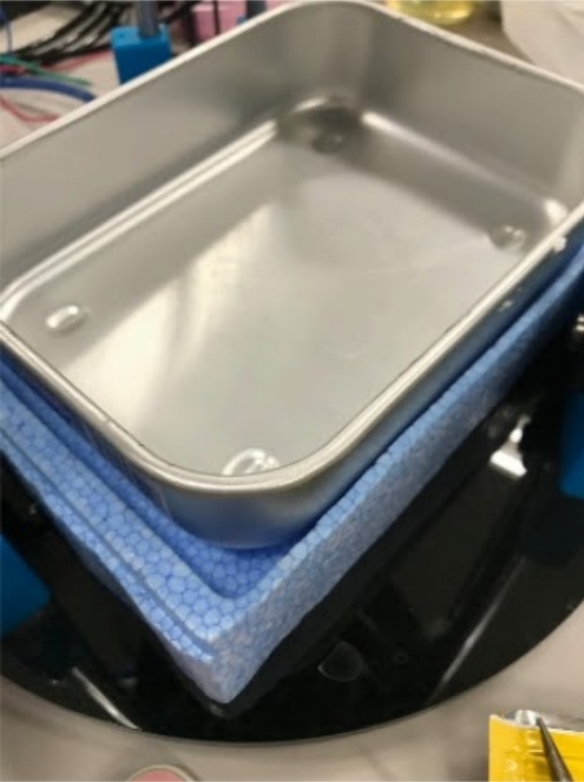
\includegraphics[width=9truecm]{./fig/yobi34.jpg}
  \caption{制作した実際の装置}
% \url{http://www.this.is.sample.url/} % Web上のデータの場合、参照先URLを明記
  \label{fig:yobipure}
\end{figure}

制作した装置は図4.3である.
この装置を使い,水の粘度がどの程度が造形速度と造形精度に影響するのか,水と粘度を上げた水を使用して比較を行った.

造形物はオーバーハングの調査を行うため図4.2のように中を空洞になるように造形を行った. 

水で造形を行った造形では,高さが 2.0mm  程のしずくがぼつぼつとある状態のものが出来上がった.
また,氷の造形物の上に積層しようと思っても,氷が水をはじいてしまい,積層ができなかった.

水の粘度を上げて造形を行ったものが図4,4である.
造形時間は約 5 分ほどで完成した.
大きさは横幅約 3 センチ,高さ約 1.5 センチほどである.使用した水の量は,約 100ml ほどである.

\begin{figure}[H]
  \centering
  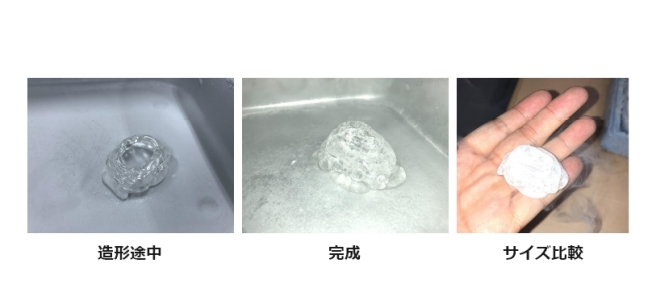
\includegraphics[width=15truecm]{./fig/yobi.jpg}
  \caption{造形過程と完成物}
% \url{http://www.this.is.sample.url/} % Web上のデータの場合、参照先URLを明記
  \label{fig:yobikekka}
\end{figure}

予備実験では,水の粘度がどの程度が造形速度と造形精度に影響するのか,調査を行った.
結果は,関連性があると考えられる.粘度を上げた水の方が,水のみに比べ造形精度が高かった.
また,速度については,水のみの造形では積層ができず比べることができなかったが,粘度のある水では、積層が可能でありオーバーハングも制作できることが確認できた.

\section{造形の仕組み}
\label{sec:paragraph}
予備実験では,液体窒素と水に砂糖を混ぜ粘度を上げることにより,リアルタイムに造形が可能になることが分かった.
ここでは,予備実験を自動化させ,プリンターが氷を積層造形していく仕組みについて解説する.
造形用のペットに熱伝導率の高い金属製のアルミプレートを使用し、液体窒素の保温性を高める為発泡スチロールでできた容器に沈めた.
液体窒素は-196℃であり,アルミプレートもそれに近い温度まで冷やされる.そこに水をたらすことで,水が冷やされ氷が作られる.
氷は,アルミプレートを通して、液体窒素により冷やされ続けるため,氷の温度も0℃以下になる,その上に水をたらすことで氷が積層される.
また,実際に制作した装置を図4.5 図4.6に示す.

\begin{figure}[H]
  \centering
  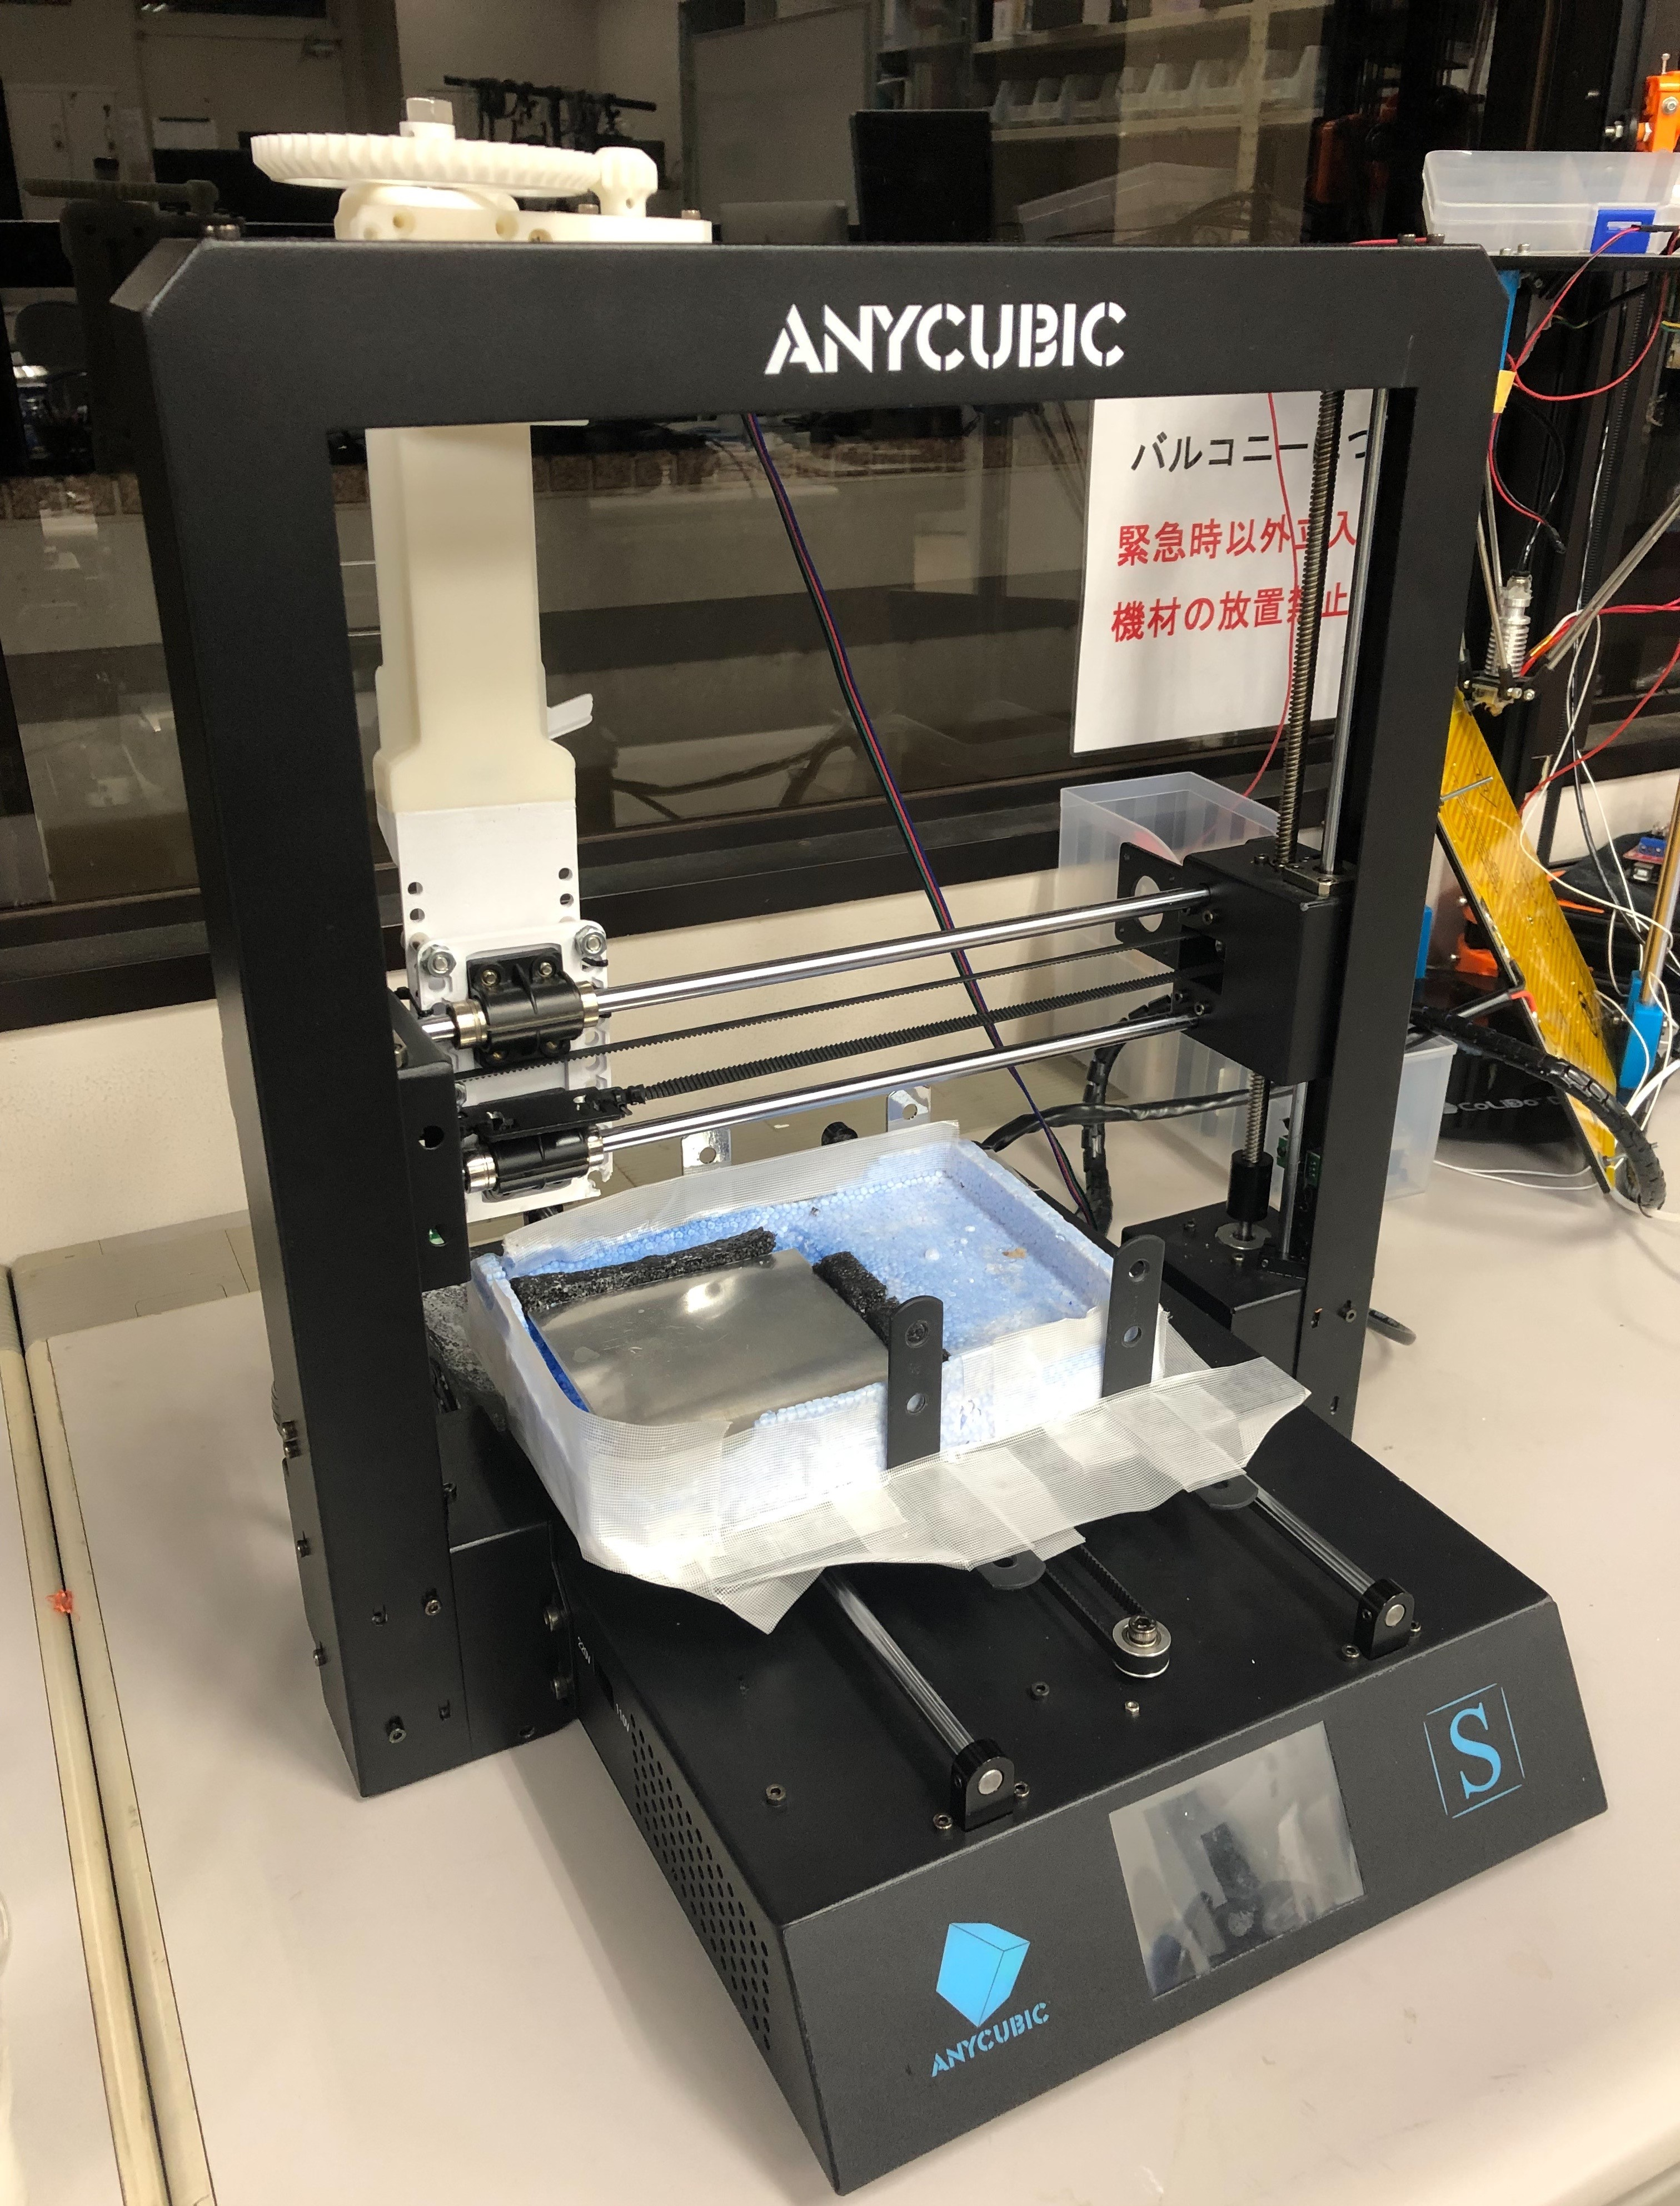
\includegraphics[width=7truecm]{./fig/printer.jpg}
  \caption{開発した氷をマテリアルとしたプリンターの全体図(前)}
% \url{http://www.this.is.sample.url/} % Web上のデータの場合、参照先URLを明記
  \label{fig:printer}
\end{figure}


\begin{figure}[H]
  \centering
  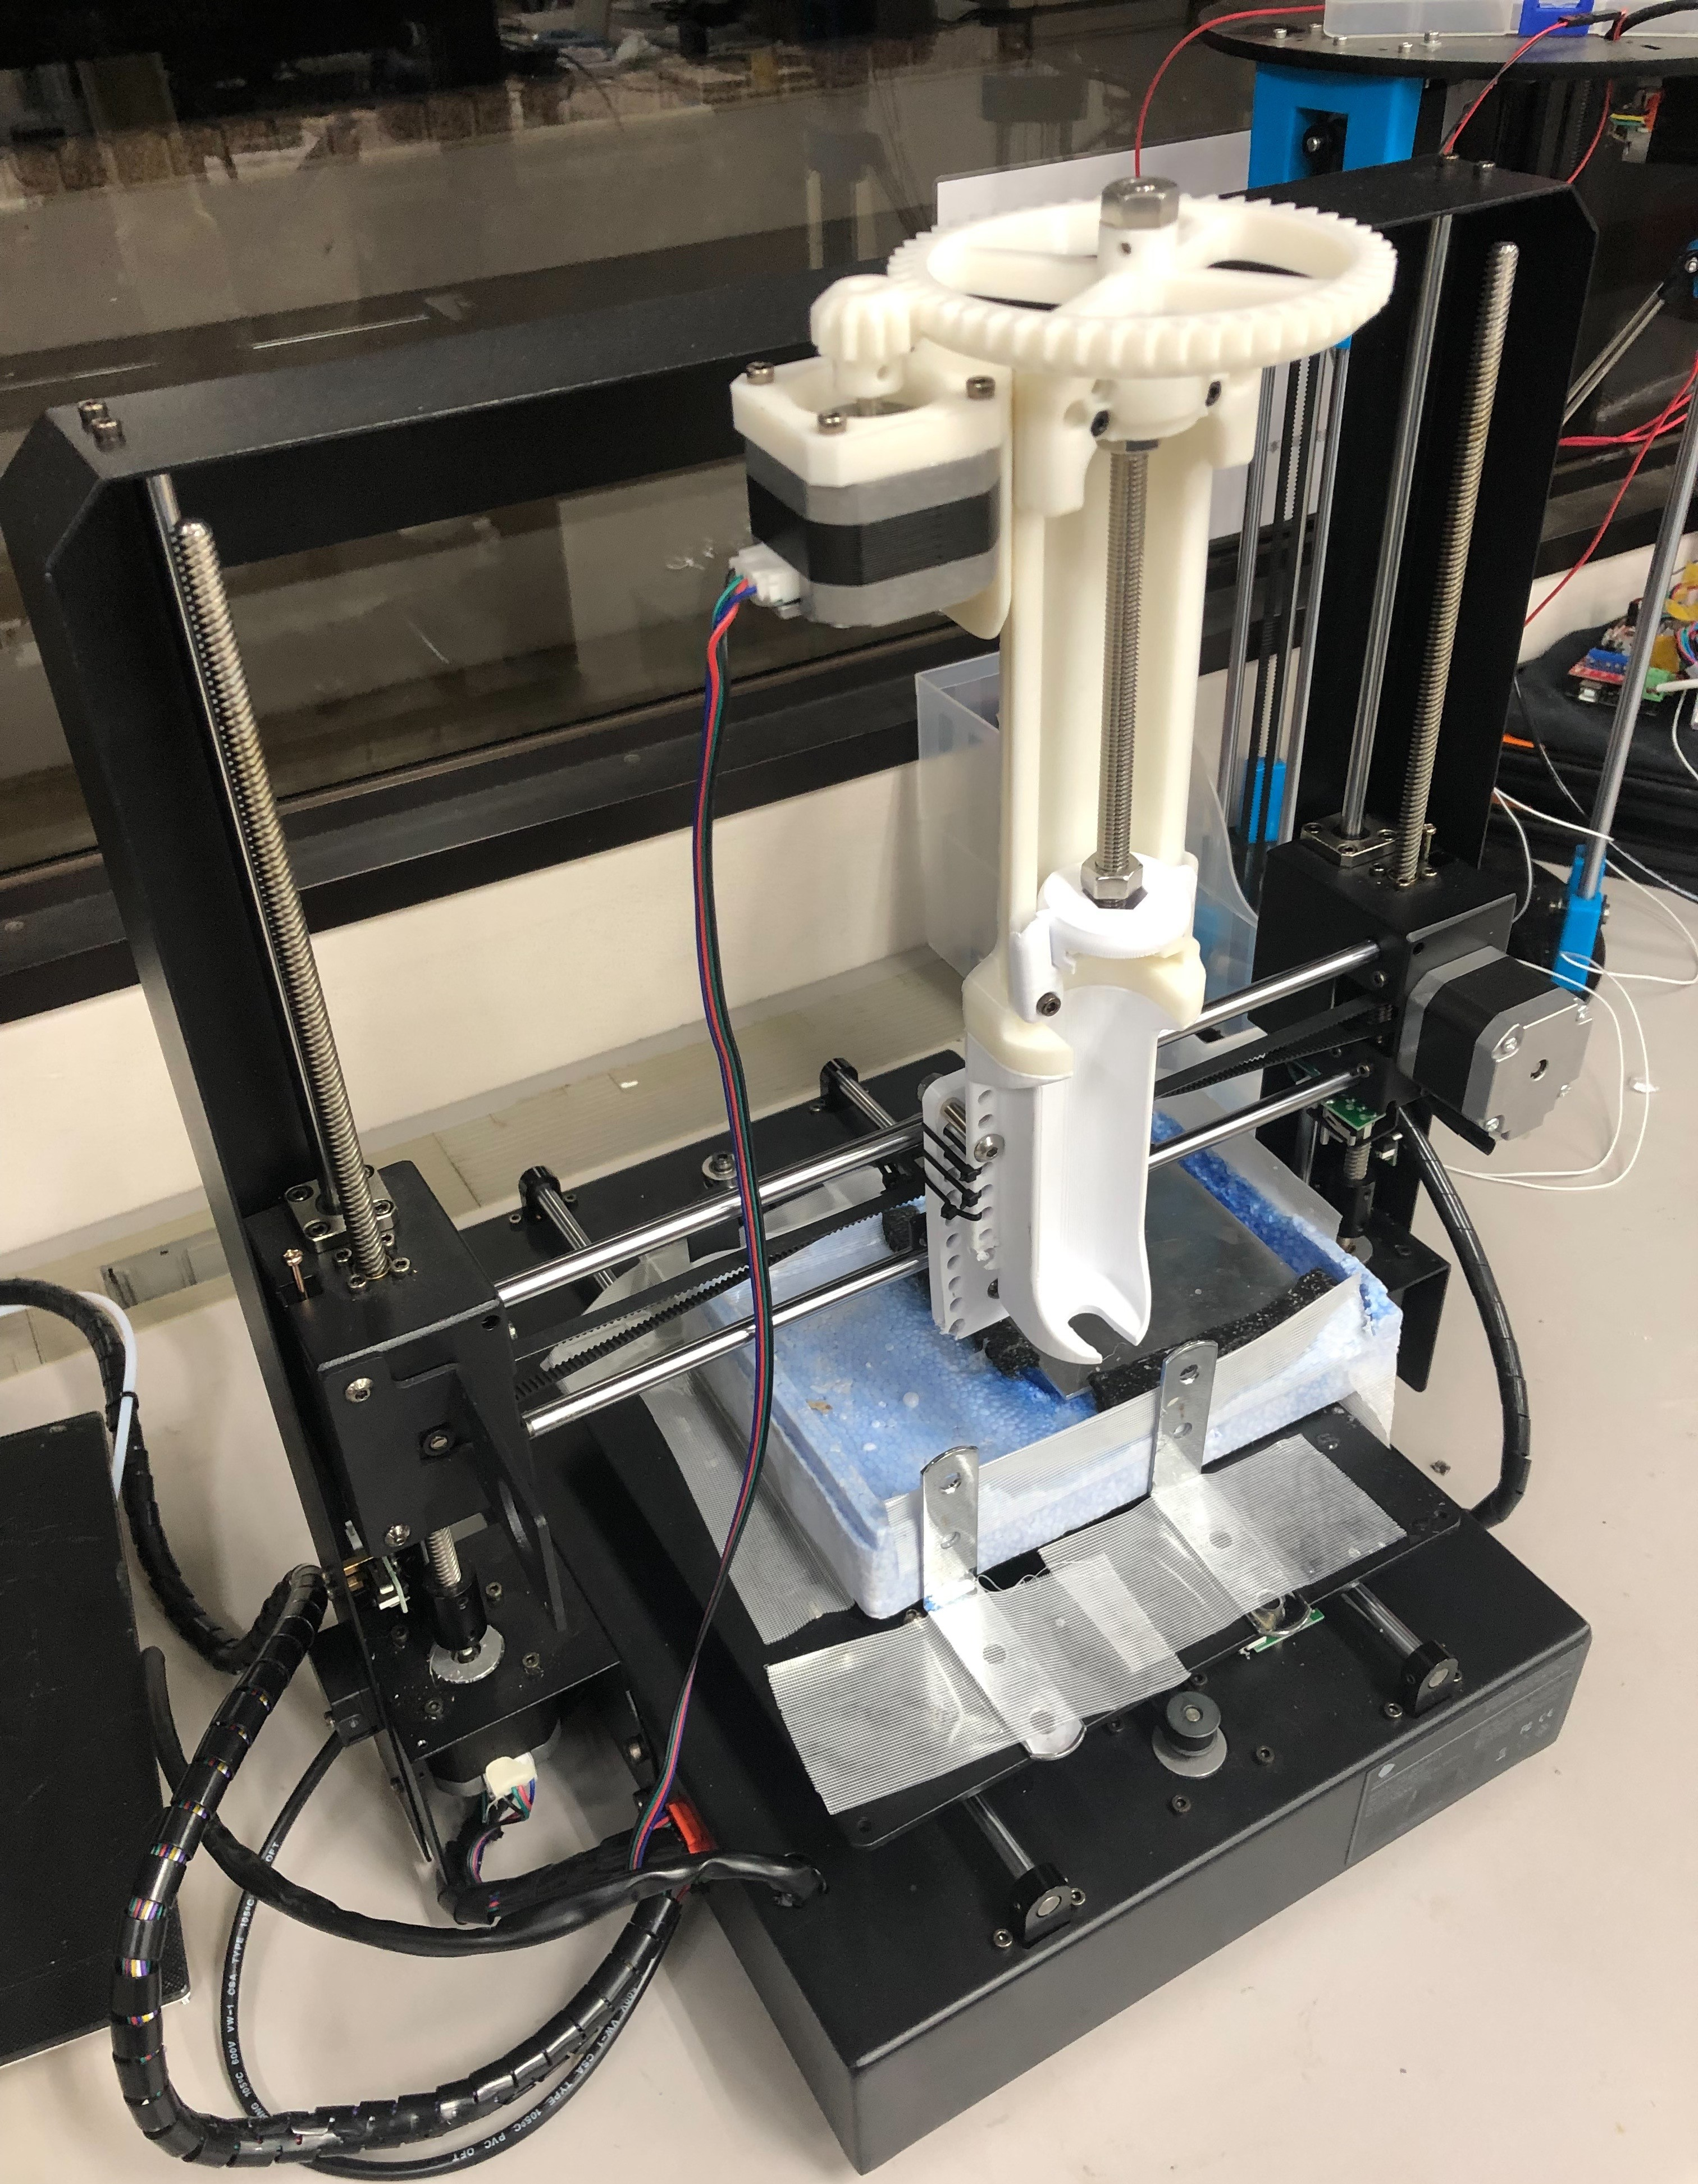
\includegraphics[width=7truecm]{./fig/printer2.jpg}
  \caption{開発した氷をマテリアルとしたプリンターの全体図(後)}
% \url{http://www.this.is.sample.url/} % Web上のデータの場合、参照先URLを明記
  \label{fig:printer2}
\end{figure}



\section{液体窒素を用いた造形の実装}
\label{sec:paragraph}
ここでは,液体窒素を使用した造形機構について述べる.
ノズルから水を供給するためのシリンジを押し出す機構を実装した.
また,今回の水は粘度を持たせているため,長いチューブを用いてしまうと,抵抗で押し出すのが難しくなる.そのためシリンジからノズルまでの距離ができるだけ短くなる機構を実装した.

\section{プリンターの本体}
\label{sec:paragraph}
3Dプリンター本体は一般に販売されているものを改造して使用した.使用した3Dプリンターは,「 Anycubic i3 Mega S 」である.

\section{プリンターの制御}
\label{sec:paragraph}
氷の3Dプリンターの制御は,Marlin-Ai3Mという3Dプリンターの制御用アプリケーションとMarilnというファームウェアを一部改造し使用している.
改造内容は,モーターの駆動方向の変更,モータードライバーへの対応,3Dプリンターは安全装置として,一定の温度以下で作動しないようになっている.
この安全装置が0℃以下で稼働する氷の3Dプリンターでは必要が無いため,無効にさせた.

今回制作したプログラムは,Ultimaker Curaを通して「 Anycubic i3 Mega S 」にアップロードさせた.
この作業を行ったことにより,基本的に一般に販売されている3Dプリンターと同じように制御することができる.

\section{シリンジの機構}
\label{sec:paragraph}
実際に制作したシリンジを図4.7に示す.
「60ml Syringe Extruder for Liquid Deposition Modeling - LDM」の機構を一部改造して制作した\cite{abc}.
シリンジを押し出して水を供給するために,既存のエクストルーダー用のモーターを利用している.
シリンジを押し出すためにモーターの回転を上下の運動へ置き換えるために、全ねじ棒を使用した.また,そのままモーターを直結してしまうと,力不足になることが想定されてため,ギアで回転数を調整している.
既存の3Dプリンターでは、フィラメントを押し出すモーターを利用しているため,PCを使い水の押し出し量を自由に調整することが可能であり,安定して造形ができる設定を模索することができる.

シリンジは3Dプリンターを使い制作したが,サイズが研究室にあるプリンターに収まりきらなかったため,上下に分割して印刷し,印刷後接着剤により合体させている.

\section{ノズルの機構}
\label{sec:paragraph}
実際に制作したノズルを図4.8に示す.
水に砂糖を加え,粘性を持たせた液体を流すため,シリンジからノズルまでの距離が長いとその間で抵抗が発生しシリンダーやシリンダー制御用のモーターに負担をかける.
そのため、できるだけ,シリンジからノズルの距離が近い方がいいと考える.
そこで,シリンジを直接ノズルとして使用し,素材を押し出せる機構を制作した.
また,ノズルサイズは今回の実験では1mmである.市販されているシリンダーの先をヒートガンで溶かし,先を塞いだ後にドリルによって穴を空けた.

\begin{figure}[H]
  \centering
  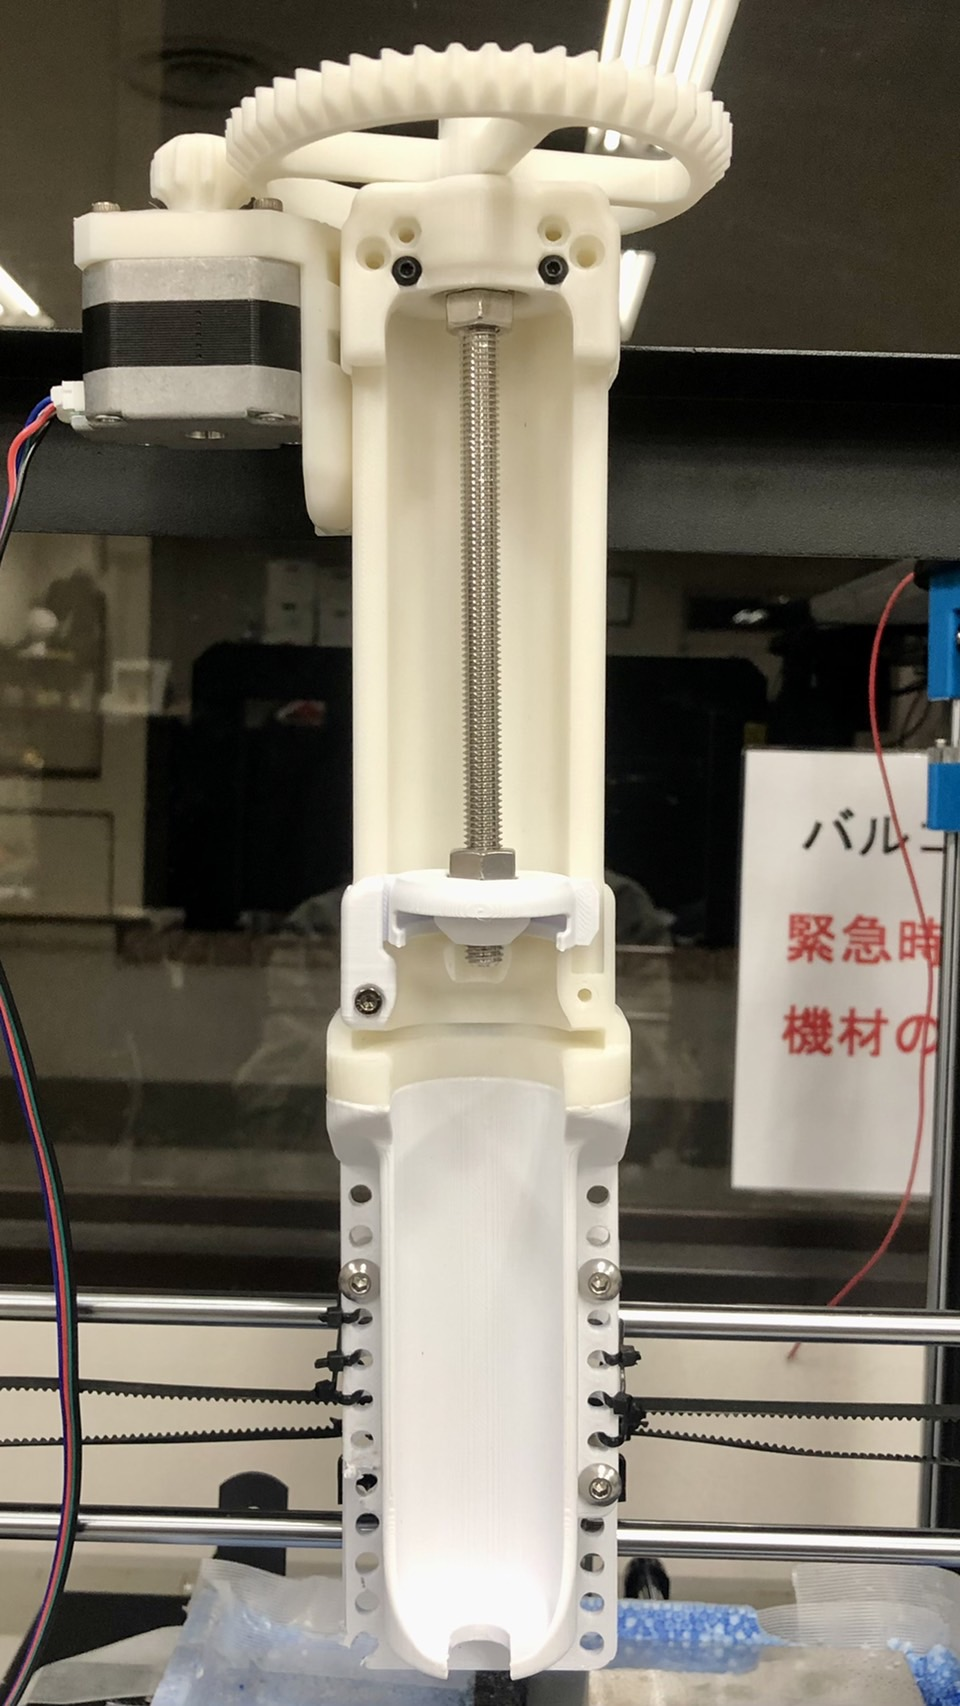
\includegraphics[width=8truecm]{./fig/101285897.jpg}
  \caption{シリンジの機構}
% \url{http://www.this.is.sample.url/} % Web上のデータの場合、参照先URLを明記
  \label{fig:printer2}
\end{figure}


\begin{figure}[H]
  \centering
  \includegraphics[width=14truecm]{./fig/sirinda.jpg}
  \caption{ノズル}
% \url{http://www.this.is.sample.url/} % Web上のデータの場合、参照先URLを明記
  \label{fig:stage}
\end{figure}


\section{ベッドの機構}
\label{sec:paragraph}
液体窒素で氷を造形するベッドとして、大きく2つに分けられる.1つ目が液体窒素用のトレーだ.液体窒素用のトレーでは,下に保温性を高め、液体窒素の持ち時間を長くするために、発泡スチロールを使用した.
また,アルミプレートの下に液体窒素がたまるようにくぼみをつけている.
2つ目が造形用のトレーだ.熱伝導率の高い金属のプレートを使用する.今回はアルミ製のプレートを使用した.
また,造形したものを取り出しやすくするために、取り外しが容易な設計を行った.完成したハードは図4.9 のようになっている.


\begin{figure}[H]
  \centering
  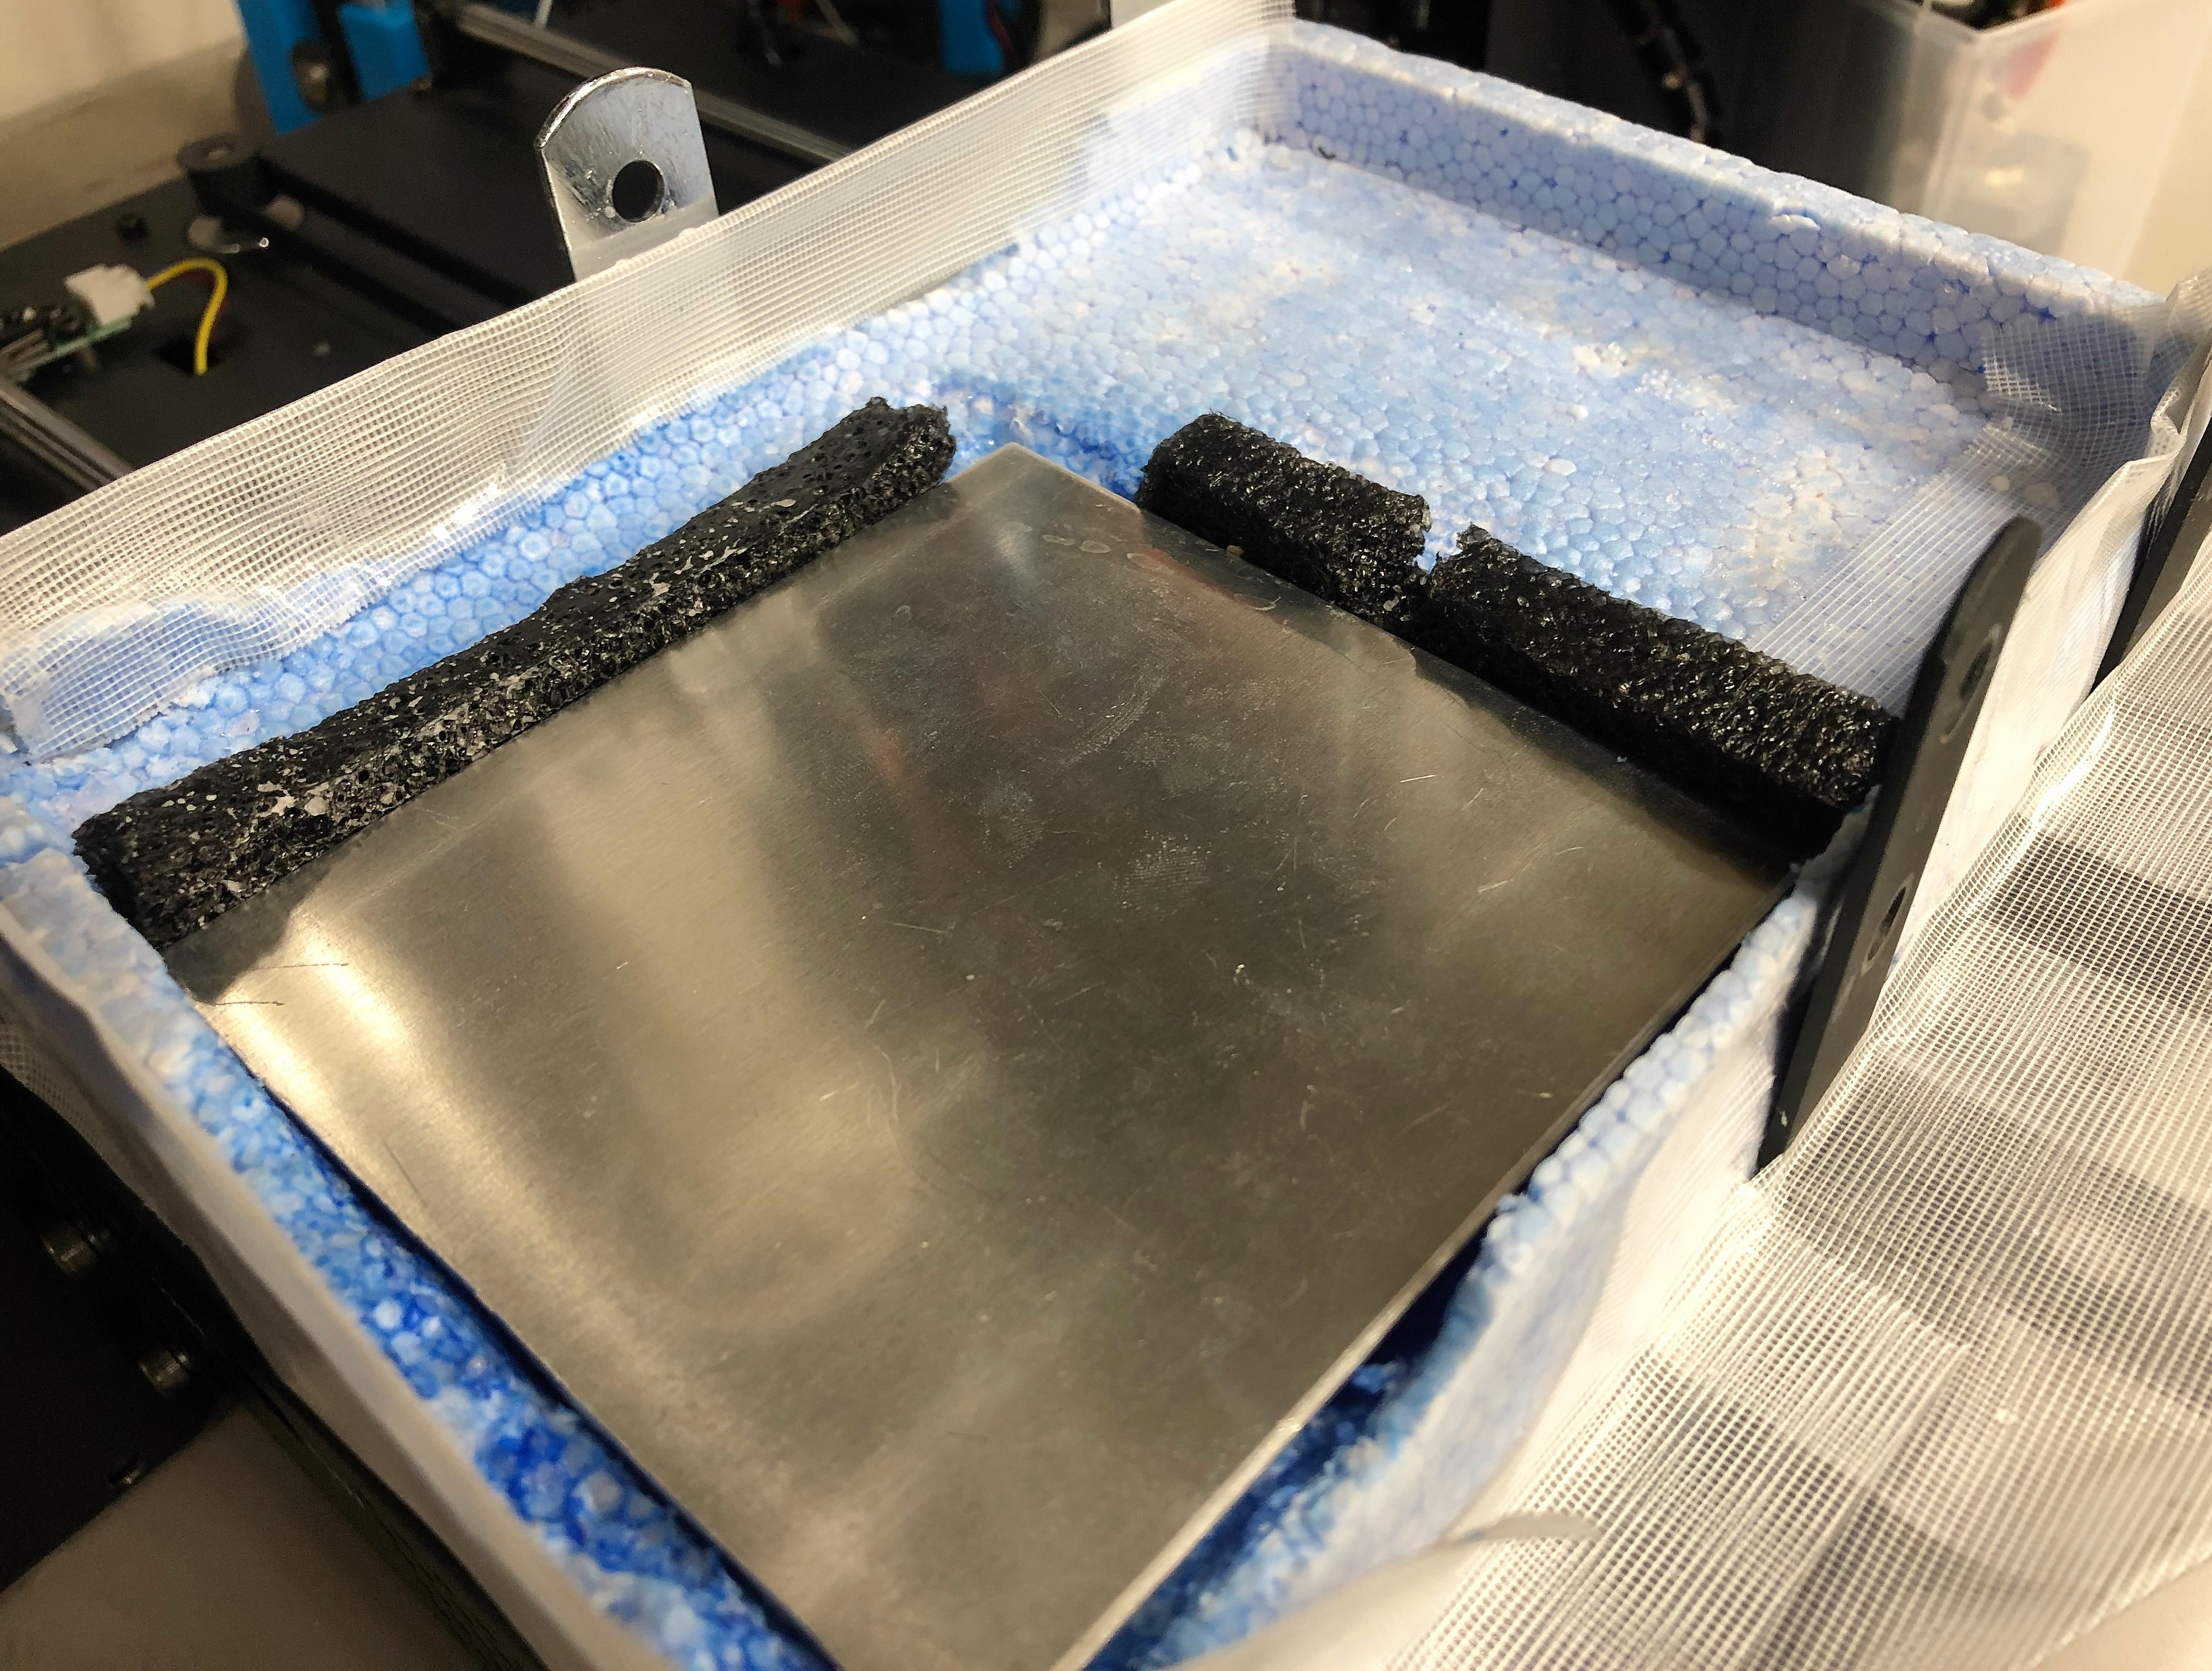
\includegraphics[width=10truecm]{./fig/stage.jpg}
  \caption{液体窒素造形用ベッド}
% \url{http://www.this.is.sample.url/} % Web上のデータの場合、参照先URLを明記
  \label{fig:stage}
\end{figure}

